%--- 11 -------------------------------%
\item\quest{Définissez ce qu’est une section critique et dans quelle situation l’existence d’une telle section peut poser problème (illustrez avec un exemple). Citez et expliquez une solution que l’on peut
apporter pour protéger de telles sections en synchronisant des processsus.}
{
 Une section critique est une ressource (donnée en mémoire, fichier,...) partagée entre plusieurs processus
\paragraph{}
Une telle section pose problème en situation de concurrence pour des \textbf{opérations atomiques}. Une op. atomique est une opération qui NE PEUT PAS ETRE INTERROMPUE
\paragraph{Exemple...}Soit deux processus, qui utilise un buffer. Le premier (producteur) ajoute un élément au buffer tant qu'il n'est pas plein et le second (consommateur) retire un élément s'il y en a un. Les deux programmes partagent une donnée \textit{counter} qui définit le nombre d'éléments présent actuellement dans le buffer.
\paragraph{}Pour mettre cette donné à jour, les programmes utilisent des \textsc{opérations de haut niveau} du type "counter++" et "counter--" qui elles-mêmes regroupent plusieurs \textsc{instructions bas niveau}. De telles opérations sont atomiques. En effet, si l'un des processus est interrompu par l'autre alors qu'il se trouvait entre deux instructions (autrement dit, l'opération counter++/-- nétait pas finie), le second va manipuler une valeur de counter qui n'est pas à jour. En fonction de l'ordre des instructions bas niveaux entre les deux processus, on pourrait donc se retrouver avec une valeur erronnée pour la donnée partagée.

\paragraph{}Afin de résoudre un problème de section critique, trois conditions doivent être respectées (simultanément):
\begin{enumerate}
\item \textbf{Exclusion mutuelle}: Si un processus est dans sa section critique, aucun autre processus ne peut y accéder en même temps. Dès lors, un processus doit demander l'autorisation à l'Os avant de pouvoir accéder à une section critique. IMAGE STRUCTURE PROCESSUS
\item \textbf{Progression}: lorsque plusieurs processus demandent l'accès à une section critique (qui n'est pas occupée), l'OS doit choisir qui va pouvoir y entrer.
\item \textbf{Attente limitée}: si un processus demande l'accès à une section critique, il devra tôt ou tard être accepté. Une demande ne peut pas être reportée à vie par l'OS.
\end{enumerate}

\paragraph{}Ainsi, dans l'exemple si dessus, si le producteur commence son opération "counter++", càd qu'il entre dans section critique puisque la valeur "counter" est partagée, le second processus ne pourra accéder à la valeur de counter tant que les instructions de bas niveau de l'opération ne seront pas toutes finies.
}


%--- 12 -------------------------------%
\item\quest{Définissez ce qu’est un deadlock et dans quelles situations il peut se produire (illustrez avec un exemple). Comment peut-on détecter, prévenir et se remettre d’un deadlock ?}
{
Un deadlock est une situation dans laquelle un ensemble de processus attend des ressources (partagées) qui sont respectivement utilisées par les uns et les autres. Chaque p. est alors en mode WAITING, formant ainsi un blocage.
\paragraph{}

Pour qu'une telle situation ait lieu, il faut que les quatres conditions suivantes soient satisfaites \textbf{simultanément}:
\begin{enumerate}\setlength{\itemsep}{.3em}
\item \textsc{Exclusion mutuelle}: au moins une ressource ne peut pas être partagée
\item \textsc{Hold and wait}: un p. détient des ressources et en attend d'autres qui ne sont pas disponibles
\item \textsc{Pas de préemption}: si le système n'est pas préemptif, une ressource ne peut pas être volontairement récupérée par l'OS
\item \textsc{Attente circulaire}: ensemble de pro. qui s'attendent les uns les autres pour récupérer des ressources
\end{enumerate}

\paragraph{}
Un \textit{graphe d'allocation des ressources système} permet d'illustrer facilement la consommation de ressources à un istant t.

\begin{figure}[!h]
\center
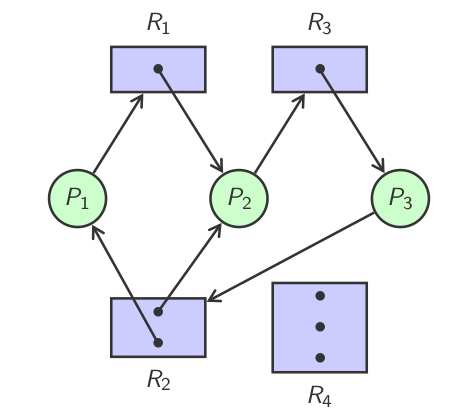
\includegraphics[scale=.3]{images/graphe-deadlock}
\end{figure}
\paragraph{}
Dans l'exemple ci-dessus, le pro P2 détient une instance de la ressource R2 et il souhaite accéder la re R3. Cette re est utilisée par P3 qui, lui, attend qu'une instance de R2 soit libérée.
\paragraph{}
Une analyse d'un tel graphe permet de tirer certaines conclusions...
\begin{itemize}
\item[$\cdot$]Si les re n'ont qu'une instance alors un cycle = deadlock
\item[$\cdot$]Si certaines re ont plusieurs instances alors on ne peut rien affirmer. Dans l'exemple précédent, les deux instances de R2 sont consommées. Comme P1 attend la re R1 détenue par R2 (qui est actuellement bloqué), aucune instance ne devrait pouvoir se libérer = deadlock.\paragraph{}Dans une autre configuration, si une des instances avait pu être libérée alors le deadlock aurait été levé tout seul après un certains temps.
\end{itemize}

\paragraph{Gestion de deadlock...} l'OS  a trois possiblités pour gérer un deadlock:
\begin{enumerate}
\item \textsc{Prévention}: l'OS s'arrange pour que le système n'atteigne JAMAIS un état de deadlock (technique particulièrement difficile à mettre en place dans le cas des syst. "grands publics")(Ex d'algo d'évitement: "banquier", "demande de ressources", "état sain")
\item \textsc{Détection}: l'OS détecte une situation de deadlock et tente de la résoudre
\item \textsc{Ignorance}: l'OS suppose qu'un deadlock n'arrivera jamais (ex: dans le cas de Linux et Windows, c'est aux développeurs de mettre les solutions en place dans leur applications)
\end{enumerate}


\paragraph{}
\textit{(Qqes algos, description état safe/unsafe, ...)}
}


%--- 13 -------------------------------%
\item\quest{Citez et expliquez les différents moyens que l’on peut mettre en oeuvre pour faire communiquer
entre eux des processus coopératifs ? Quels sont les avantages et inconvénients de ces deux
moyens de communication ?}
{}


%--- 14 -------------------------------%
\item\quest{Expliquez ce qu’est le principe d’adressage ? Comment l’unité mémoire intervient-elle ? Définissez et expliquez le principe de liaison des adresses.}
{
Adressage: façon dont sont accédées les données stockées en mémoire. La mémoire est un grand tableau d'octets qui sont identifiés par une adresse unique. 

\paragraph{}
Lors de l'exécution d'une instruction par le CPU, des données sont \textbf{chargées depuis} la mémoire ou \textbf{stockées vers} la mémoire. Pour accéder à la bonne zone de la mémoire, il faut alors préciser son \textit{adresse mémoire}.

\paragraph{L'unité de gestion mémoire (MMU)}
\paragraph{}
On distingue deux types d'espaces d'adresses:
\begin{enumerate}
\item Adresse \textsc{physique}: adresse de la donnée dans la mémoire physique (RAM ou disque)
\item Adresse \textsc{logique} (ou \textsc{virutelle)}: adresse de la donnée au sein de la mémoire virtuelle propre au processus.
\end{enumerate}
\paragraph{}
L'unité mémoire, elle voit défiler un flux d'adresses et elle est chargée de faire la conversion entre les deux types ci-dessus. \textbf{\textit{Rem:}} elle ne fait que répondre aux demandes, sans interpréter les adresses fournies. L'aspect sécurité est implémenté au niveau hardware et n'est donc pas de sa responsabilité.


\paragraph{Principe de liaison des adresse}
}


%--- 15 -------------------------------%
\item\quest{En quoi consiste le swapping ? Citez et expliquez les différentes formes de swapping qu’il existe, et comparez-les.}
{
Le \textit{swapping} consiste à déplacer, temporairement, hors de la mémoire RAM un processus afin d'y libérer de l'espace. Le processus de l'OS qui est en charge des swaps est le \textbf{dispatcher}.

\paragraph{}
On distingue principalement deux formes de swapping:
\begin{enumerate}
\item Le swap d'un \textsc{processus entier}: l'entièreté du processus est déplacé vers l'espace de stockage de masse (disque dur)
\item Le swap d'une \textsc{partie de processus}: certaines parties du processus, dites "pages", sont déplacées. De cette façon, le p. peut encore fonctionner avec les pages restantes en RAM. On peut parle de \textit{pagging}.
\end{enumerate}

\begin{figure}
\center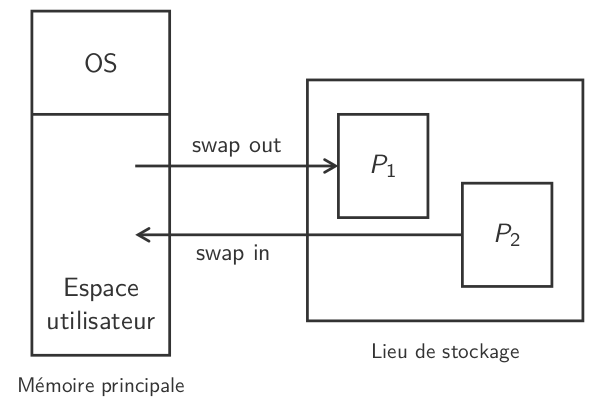
\includegraphics[scale=.3]{images/swapping}
\end{figure}

\paragraph{}
Il est a noter que ce déplacement de données nécessite un certains temps qui dépend de la vitesse de transfert (temps perdu point de vue utilisateur). Dans un ordinateur bien configuré et avec suffisamment de RAM, cette opération de swapping ne devrait jamais avoir lieu avec un usage normal.
\paragraph{}
De plus, si un p. est swappé alors qu'il est attente d'une E/S, lorsque celle-ci sera disponible il devra soit être swappé immédiatement en mémoire RAM soit le résultat de E/S devra être stocké en RAM en attendant le retour du p. (perte de place)
}


%--- 16 -------------------------------%
\item\quest{Citez, expliquez et comparez les différentes stratégies d’allocation de la mémoire que l’on peut mettre en place. Quels sont les risques de fragmentation liés à ces stratégies ?}
{}


%--- 17 -------------------------------%
\item\quest{Expliquez le principe de la segmentation. En quoi est-il plus proche de la pensée du programmeur? Comment les adresses sont-elles construites lorsqu’on utilise la segmentation ?}
{}


%--- 18 -------------------------------%
\item\quest{Expliquez le principe de la pagination. Quels sont ses avantages par rapport à la segmentation? Comment les adresses sont-elles construites lorsqu’on utilise la pagination ? Comment peut-on améliorer les performances de la pagination à l’aide d’une mémoire spécialisée ?}
{
La \textit{pagination} est une technique d'allocation de la mémoire aux processus qui consiste à découper la mémoire logique ( = mémoire virtuelle propre à chaque processus) en \textbf{pages} de même taille et à découper la mémoire physique ( = RAM ) en \textbf{cadres} de taille fixe. Un cadre est alors rempli par une page et une table des pages (propre à chaque p) permet d'associer les pages aux cadres.

\paragraph{}
En pratique, l'entièreté d'un processus n'est jamais requise au même moment, stocker l'ensemble de ses données en RAM représente donc une perte de place conséquente. En utilisant la technique de pagination, on divise la mémoire du processus et on ne charge en RAM \textbf{que ce qui est nécessaire} à son fonctionnement à un instant t. Les pages restantes sont alors stockées sur la mémoire de masse et chargées dynamiquement à la demande.

\begin{figure}[!h]
\center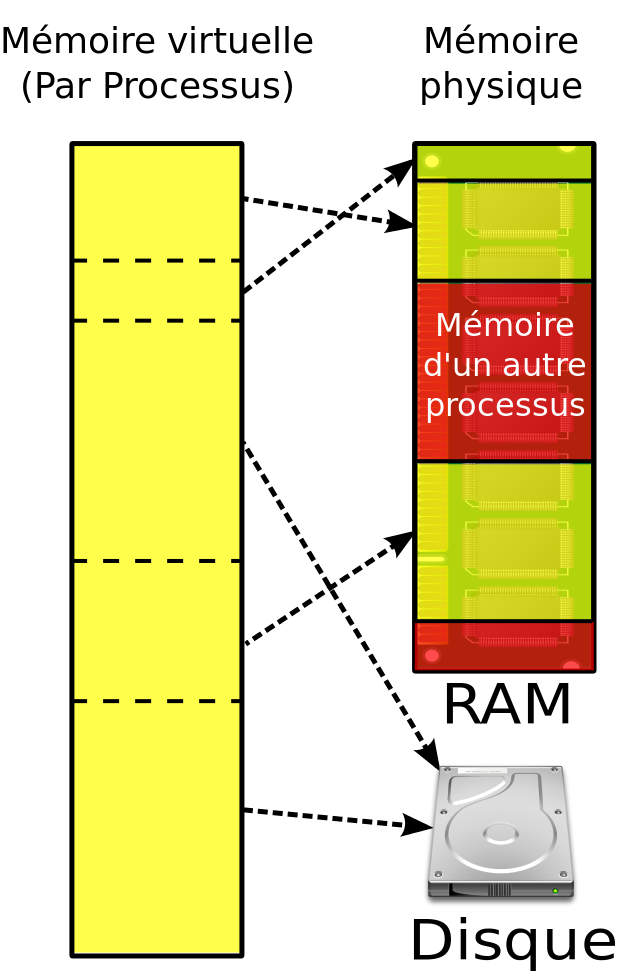
\includegraphics[scale=.2]{images/memoire-virtuelle}
\end{figure}

\paragraph{Calcul des adresses}
\paragraph{}
Pour identifier une donnée au sein de la mémoire virtuelle, on utilise son \textbf{adresse logique} qui est composée d'un couple <\textit{numéro de page}, \textit{décalage}>

\begin{figure}[!h]
\center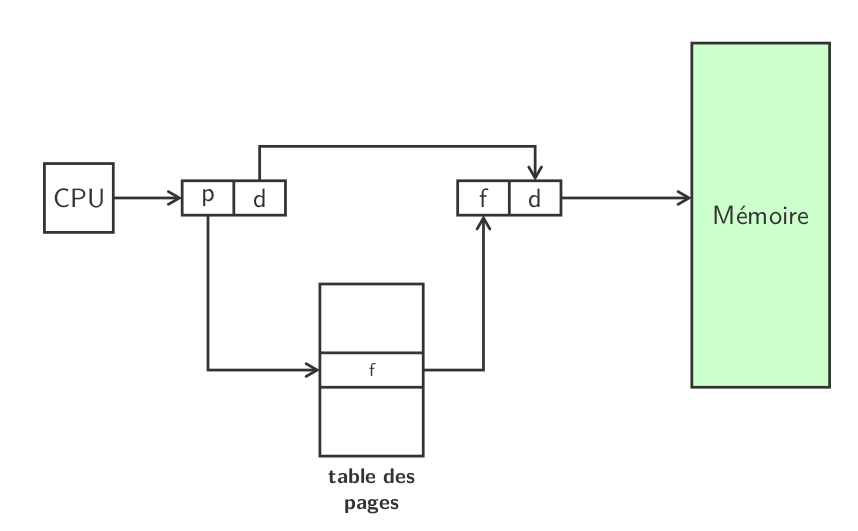
\includegraphics[scale=.3]{images/calcul-adresse-pagination}
\end{figure}

Lorsque le CPU émet une adresse virtuelle (logique), la table des pages fait correspondre le numero de la page avec le cadre (adresse physique) dans lequel elle est stockée et le décalage permet de se positionner au sein cette zone de mémoire.
}


%--- 19 -------------------------------%
\item\quest{Citez et expliquez les différentes structures que l’on peut utiliser pour stocker la table des pages.
Quels sont les avantages et inconvénients de ces structures ? Dans quelles situations sont-elles
plus adaptées ?}
{}


%--- 20 -------------------------------%
\item\quest{Définissez et expliquez les différences et les liens entre mémoire physique et mémoire virtuelle. Comment le système d’exploitation fait-il le lien entre ces deux mémoires, pour les différents processus ?}
{}